\chapter{GUI}

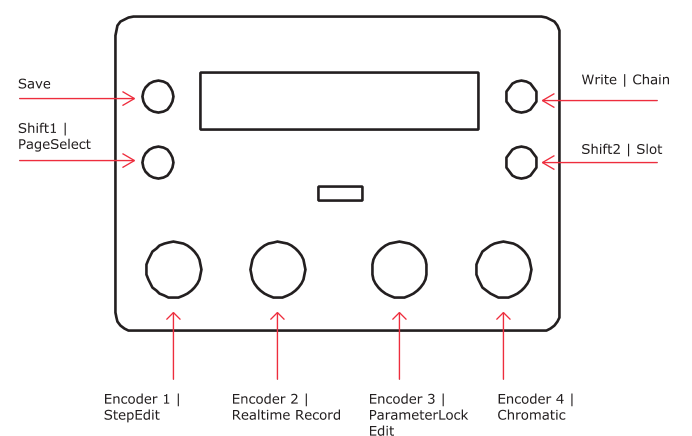
\includegraphics[scale=.6]{mcl_gui.png}\\
The MegaCommand's four upper function buttons are used to enter submenus and activate commands:
\section{Function Buttons:}
From the Grid Page the function buttons perform the following actions:
\begin{itemize}
\item{\textbf{[Save]}: Enters the Save Page}
\item{\textbf{[Write | Chain]}: Enters the Write or Chain page}
\item{\textbf{[Shift1 | PageSelect]}: Enters the PageSelect page}
\item{\textbf{[Shift2 | Slot]}: Opens the slot Menu }
\end{itemize}
Combined Button Presses:
\begin{itemize}
\item{\textbf{[Save] + [ Write | Chain ]}: Opens the Global Settings menu }
\end{itemize}

\section{Encoder Buttons}
From the Grid Page the encoder buttons are used to access Sequencer Pages:
\begin{itemize}
\item{\textbf{[Encoder 1]}: Enter sequencer StepEdit page}
\item{\textbf{[Encoder 2]}: Enter sequencer RealTimeRecord page}
\item{\textbf{[Encoder 3]}: Enter sequencer ParameterLock page}
\item{\textbf{[Encoder 4]}: Enter sequencer Chromatic page}

\end{itemize}

\section{Page Select}

The PageSelect page is accessed by holding the \textbf{[Shift1 | PageSelect ]} button.
\\
\\
\fbox{
\includegraphics[scale=.4]{page_select_page.png}}\\
The PageSelect page allows quick access to auxillary pages not accessible through the main GUI buttons.
When open, the PageSelect page displays the Page to be loaded, releasing \textbf{[Shift1 | PageSelect]} will load
the selected page.
\\
\\Rotating \textbf{[Encoder 1]} will scroll through the available PageSelect pages.
\begin{itemize}
	\item{1. Mixer Page}
	\item{2. Cue Page}
    \item{8, Wav Designer}
\end{itemize}
\textit{The MD's trigger interface can be used to quickly toggle between pages in the PageSelect page. }
\section{Trigger Interface}
When connected to the Elektron MachineDrum, MCL will use the MD's 16 trigger buttons as additional GUI input. \\
\\
Depending upon the current page, the Trigger Interface (TI) can be used to work in a variety of ways.
For example, the TI can be used to enter sequencer data in to the internal sequencer;
to select multiple tracks in the Mixer window and attenuate their volume simultaneously; to save or load Grid Slots from the Save or Write/Chain pages and much more.

\section{Trigger Interface Limitations}
The MD TI is not natively supported by the MD and is instead achieved using a Global Slot/MIDI Channel exploit. The exploit is used to differentiate between notes triggered by the sequencer and notes triggered by a user key-press.\\
\\
The TI will cease working whenever the MD display is updated unexpectedly, for example, when a machine parameter's value is changed; or when a submenu on the MD is opened.\\
\\
As a precaution, whenever entering a Page on the MC that uses the TI, the MD track will be automatically changed to track 16. This avoids unexpected display updates, that may be caused 
by transmitted Parameter Changes. Parameter Locks on Track 16 will therefor not be transmitted when the TI is active.\\
\\
\textit{Recovery: If the Trigger Interface stops working exit all submenus on both the MD and MC. On the MD press [ Func + Extended ] to reset the state of the MD.}





